\bartchapterimage{rampressure}
\chapter[MAGGIE]{MAGGIE\@: Models and Algorithm for Galaxy Group,
Interlopers and Environment}
\bartthumb{maggie.jpg}

\section{Introduction}
\label{sec:maggie_introduction}

We show in the last chapter that the most used galaxy group algorithm that
is the FoF should be optimized against its linking lengths, and that it
depends on the scientific goal of the group catalog obtained. With these
limitations, it is clear why Bayesian methods appeared. Indeed, with our
knowledge of the galaxy formation and evolution processes, it is possible to
constrain better the galaxy grouping. With the FoF algorithm, galaxies are
selected in a pure geometrical way, and their formation history doesn't
matter in this selection, since only the over-density is relevant. With
Bayesian algorithms, it is possible to combine geometrical and physical
approaches. The history of galaxies is available by their observable
properties such as luminosity, stellar mass, morphology and is used to
assign galaxies to a group, in complement of the geometrical information
from the density. In particular, a galaxy can be rejected of a group
selected by density criterion if its properties don't reflect the history it
would have inside this group.

We already described Bayesian algorithms in
\bartrefchapter{galaxy_group_algorithms}, for example \citet{Yang+07} or
\citet{MunozCuartas+12}, where similar spatial methods to the FoF are
adopted, with priors as the density profile of galaxies inside halos to
constrain the assignation. But because of observational uncertainties, model
divergences, various incompletenesses\ldots, the extraction of groups from
observational data will always be affected these problems, and the galaxy
environment polluted by interlopers, creating biases in group
characteristics. This leads to bad modulation of galaxy properties with
their environment and a falsification of our understanding of intra-groups
physical processes.

Recently, with the improvement of computer capacities in terms of memory and
power, it becomes possible to include many priors in the computation, and to
use the most computation intensive applications of statistics. Since
interlopers will still be problematic, the new powerful computer era allowed
probabilities to describe the membership of galaxies in groups. Systematic
errors in galaxy surveys can be reduced or integrated in the grouping by
probabilities. For example, \citet{Liu+08} used a probabilistic FoF in
galaxy survey with photometric redshifts to avoid the uncertainties
inherent to this method. \citet{DominguezRomero+12} also used
responsibilities to improve the assignation of galaxies to groups and
reduce interlopers effect on their observable properties. In
\citet{Rykoff+14}, galaxies have their probabilities based on the group
richness estimations.

It seems that using probabilities to describe the membership inside galaxy
groups will inevitable, because of the systematic errors and biases presents
in the actual and future galaxy surveys. In particular, the modulation of
the galaxy properties with their environment that we want to extract from
galaxy group catalogues should be less biased by interlopers if we use
probabilities as a weight. Indeed, interlopers, even if they are still
present in the group membership, will have a low probability to pertain to
the group.

Here is the starting point of our galaxy group algorithm called MAGGIE\@:
Models and Algorithm for Galaxy Group, Interloper and Environment. We
combine our understanding from the galaxy formation, using various models,
to compute a probability for galaxies to belong to a peculiar group, and use
it in the algorithm for the group extraction. Then interloper effects should
be reduced in the characterization of the environment.

In the following sections, we will describe the algorithm and its

\section{Algorithm}
\label{sec:algorithm}

\subsection{Description}
\label{sub:maggie_description}

MAGGIE doesn't affect a galaxy to an
unique group, but it affects a probability for this galaxy to be in a group.
With this principle, a galaxy is assigned to more than one group. It's the
goal of MAGGIE\@: to obtain the properties of galaxy groups in statistical
and probabilistic senses. This allows users of catalogues generated by
MAGGIE to compute some properties of groups taking into account the fact
that a galaxy could not be assigned arbitrarily to one group with some
criteria of affectation. But the most important, it's that this probability
contains the information of being an interloper or not.

MAGGIE is organized in an iterative way in order to be self-consistent with
the data being analysed, as for learning algorithms. For this reason, we
will describe the implementation of the algorithm in different steps. In
what follows, we assume that we have a galaxy sample with
positions (right ascension RA, declination DEC), redshifts, stellar masses,
apparent magnitudes in a given band and absolute magnitudes. It's the
minimum set of data necessary.
%
\begin{enumerate}
    \item We first get some potentials groups in order to have a \emph{seed}
        in the iterative process. For this, we make an assumption: the most
        massive galaxies (in stellar mass) are potential group centers. In
        an other implementation, we use the luminosity of the central (the
        reason is explained in \note{Add the reference to section}). But,
        some intra-group physical process can lead to a false detection of
        the brightest galaxy as the central one \citep{Ebeling+13}. From the
        galaxy sample, we sort by decreasing stellar mass (or luminosity)
        all galaxies and we start with the most massive as centre of a
        potential group.

    \item\label{step:2} For all our potential groups, we need to get our
        potential members. We are just interested in the virial sphere of
        groups. Since the unique information on groups at this step is the
        central galaxy, we use its stellar mass. At first iteration, we use
        the relation between halo mass and central stellar mass from
        \citet{BCW+10}, we used other models later to see the influence of
        this choice (\note{Add reference to section}). For next iterations,
        we use the same relation, but learned from our previous iterations.
        We can estimate the virial radius of the group assuming
        that the halo mass corresponds to the virial mass. Then, we select
        all galaxies in a cone generated by an angular separation
        corresponding to the virial radius physical size at the group's
        redshift (the redshift of the central galaxy).

    \item With group membership, we compute galaxy probabilities to belong
        to it. The probability is computed assuming a density profile of
        galaxies in groups, and a velocity distribution. Considering that
        galaxies form in dark matter halos, the density profile of
        galaxies in groups must follow a NFW distribution \citep{NFW+97}
        which fit remarkably well the dark matter particles distribution in
        $\rm \Lambda$CDM simulations. The detailed computation of the
        probability is provided in \bartrefsection{probability}.

    \item We compute the weighted (by probability) stellar mass and
        luminosity of groups. For this we use a probability threshold to
        decide if a galaxy is associated to a group, i.e.\ if we take the
        galaxy for the estimation of the group stellar mass and luminosity.
        This parameter will be optimized by tests. The way of computing this
        properties for a group is the following: we sum, using the
        probability weights, luminosities and stellar masses of galaxies
        that have an absolute magnitude less than the limit magnitude
        defined by the sample, in order to be complete.

    \item Using the stellar mass of the central galaxy, we can estimate the
        halo mass of the group. We use the abundance matching technique
        which assumes that there is a one-to-one relation between the
        central stellar mass of the group and its halo mass. It allows to
        compare the cumulative distribution function (CDF) of the two
        masses. Indeed, with this assumption, the number of groups above a
        given central stellar mass is the same than the number of groups
        above the corresponding halo mass. If we consider a certain halo
        mass function, we can predict the halo mass of a group with a given
        central stellar mass by comparing the CDF of the data with that
        predicted by the halo mass function.

    \item With the halo mass found for group by this abundance matching, we
        go back to step~\ref{step:2} and recompute groups with the halo
        mass-central stellar mass relation previously obtained. This process
        goes until there is a convergence in the number of groups.
\end{enumerate}

\section{Probability}
\label{sec:probability}

\section{Results on mock catalogue}
\label{sec:results_on_mock_catalogue}

\section{Application to SDSS}
\label{sec:application_to_sdss}



\section{Flux-limited algorithm}

\subsection{Problem}

For MAGGIE, we tried to create a flux-limited version of the algorithm to
apply it in a large range of luminosities and redshift.

The problem is that we must correct for missing galaxies. One way is to take
into account the luminosity function of galaxies in the sample, and with
that assumption, correct for the fraction of missing galaxies expected at a
given redshift. Assuming that the luminosity function is
$\phi\left(L\right)$, this fraction can be written:
%
\begin{equation}\label{eq:correc}
    f\left({L_{\lim}{\left({z}\right)}}\right)=\frac{\int_{L_{\lim}\left({z}\right)}^{\infty}L\phi{\left({L}\right)}\dd{L}}{\int_{L_{thres}}^{\infty}L\phi{\left({L}\right)}\dd{L}}
\end{equation}
%
where $L_{\lim}\left({z}\right)$ is the minimal luminosity that a galaxy should
have to be observed at the redshift $z$, given the observed magnitude limit
$m_{\lim}$ of the survey, in the used wavelength range:
%
\begin{equation}
    L_{\lim}\left({z}\right)={{\left(\frac{d_{\rm{lum}}\left({z}\right)}{10pc}\right)}^2}10^{0.4\left({M_{\odot}-m_{\lim}}\right)}
\end{equation}
%

We expect the galaxy environment to modulate galaxy properties such as their
luminosity. Correcting for missing galaxies in all groups in the same way is
in consequence ideal. We can modulate the luminosity function with the host
halo of the galaxy by transforming the luminosity function into a
conditional luminosity function. Since our estimations of the virial mass
$M$ of the host halo is good, we can use it as modulation parameter an so:
%
\begin{equation}
    \phi\left({L}\right)\rightarrow\phi\left({L|M}\right)%
\end{equation}

\subsection{Environment modulation}

In galaxy groups, we separate galaxies in two classes: centrals and satellites.
Centrals are expected to be the most massive galaxies in groups, and
consequently, it's probable that the central is the brighter galaxy. A
consequence is that if we can't see the central galaxy, we can't see other
galaxies in the group and the correction is not needed because we don't know
how to correct for incompleteness. So for the correction we just need to
constrain the distribution of luminosities in satellite galaxies.

In practice, we have to choose a functional for this conditional luminosity
function (CLF) which can be easily fitted and integrated to determine the
correction factor in our group luminosities.

There are two kind of luminosity function widely used. The Schechter
function can be written as:
%
\begin{equation}
    \phi\left(L\right)=\phi^*{\left(\cfrac{L}{L_*}\right)}^\alpha
    \exp\left(-\left(\cfrac{L}{L_*}\right)\right)
\end{equation}
%
where $\alpha$ characterizes the slope in log-space of the function, $L_*$
the luminosity of turn-off and $\phi^*$ is the normalization of the
function.

In studies of the galaxy sample from the SDSS survey as in
\citet{Blanton+05}, the LF has been well fitted by a double Schechter
functional form which can be written:
%
\begin{equation}\label{eq:dblsch}
    \phi\left({L}\right)=\left({\phi_1^*{\left({\cfrac{L}{L_*}}\right)}^{\alpha_1}+\phi_2^*{\left({\cfrac{L}{L_*}}\right)}^{\alpha_2}}\right)\exp\left({-\left({\cfrac{L}{L_*}}\right)}\right)%
\end{equation}
%
This model uses the fact that it seems to exist two galaxy population in
luminosity a brighter one and a low one.

Now we assume that the CLF have the same form that (\ref{eq:dblsch}). The
dependence on the halo mass $M$ is done with the parameters of the double
Schechter (DS). For example
$\alpha_1\rightarrow\alpha_1\left({M|\theta}\right)$, where the functional
form of this dependence is not given explicitly here, and $\theta$ is a set
of parameters relative to the function used to describe the dependence with
halo mass. The number of parameters in $\theta$ can vary greatly, depending
on the function used.

The form of this dependence can't be determine in advance when we want to
fit the CLF on the data. For example in the SDSS, we have to know in advance
the properties of the groups in order to choose a dependence for the
parameters of the DS with the virial mass. For testing the viability of this
method, we have to select a functional that describes correctly the
modulation of the parameters with the halo, and samples of galaxies that can
give us these informations are present in outputs of semi-analytical models
(SAM). To validate this method of correction for incompleteness, we test it
in mock galaxy catalogues.
%
\subsection{Estimating parameters}
%
When working with distribution function, it is common and better to use the
maximum likelihood estimation.
%
\remark{%
We consider a set of independent data $\left\{X\right\}$ drawn from distribution
following the probability distribution function $p$, dependent of parameters
$\theta$. If we assume that observations are independent and identically
distributed, the probability to obtain the given set of observations given
the parameters $\theta$ is just the joint probability function of the
observations. We define it as the likelihood function:
%
\begin{equation}\label{eq:like}
    \mathcal{L}\left({\theta|X}\right)=\prod_i{p_i\left({X_i|\theta}\right)}
\end{equation}
%

To obtain the most probable parameters allowing the probability function $p$
to correctly fit the data, we need to find the given set of parameters
$\theta$ maximizing the likelihood function.

If we consider Bayesian statistics, the likelihood is defined as
$p\left({X|\theta}\right)$ and the Bayes's theorem gives that we need to
maximize for the given set of data:
%
\begin{equation}
    p\left(\theta|X\right)=\cfrac{\prod_i{p_i\left({X_i|\theta}\right)}p\left(\theta\right)}{p\left(X\right)}
\end{equation}
%
where $p\left(\theta\right)$ is the prior distribution of the parameters and
$p\left(X\right)$ is the probability to obtain the set of data. But we can
see that \emph{our} likelihood is in reality the posterior distribution
which is proportional to the likelihood in the definition of Bayesian
statistics, multiplied by a prior. If we take a constant for the prior
(probability equal for each value of the parameter), since the probability
to obtain the data is constant, using directly the likelihood defined
in~\ref{eq:like}, the obtained parameters after the maximization are the
same.

Numerically, it's more convenient to use the logarithm of the likelihood in
order to prevent numerical problems when calculating the likelihood and the
product in (\ref{eq:like}) becomes a sum. Often, numerical methods for
optimization minimize of function instead of maximizing it so we put a minus
sign in front of it:
%
\begin{equation}\label{eq:loglike}
    -\log\mathcal{L}\left({\theta|X}\right)=-\sum_i{\log\left({p_i\left({X_i|\theta}\right)}\right)}
\end{equation}
%
}
%

We define $p_i\left({L_i|\theta}\right)$ as the probability to get the luminosity $L_i$
given the parameters $\theta$, so it's the probability density. To determine
this density, we need to calculate the number of galaxies in the sample which
are between $L_i$ and $L_i+\dd{L_i}$ compare to the total number of points in
the set:
%
\begin{equation}
    p_i\left({L_i|\theta}\right)\dd{L_i}\dd{V} = \cfrac{\dd^2{N_i}}{N_{\mathrm{tot}}}
\end{equation}

By definition of the CLF, which is the number of galaxies in the sample
comprised between $L$ and $L+\dd{L}$ at a given halo mass $M$, we can write:
%
\begin{equation}
    \dd^2{N}=\phi\left({L|M}\right)\dd{L}
\end{equation}
%
So we can write:
%
\begin{equation}
    p_i\left({L_i|\theta}\right)\dd{L_i}\dd{V} =
    \cfrac{\phi\left({L_i|M}\right)}{N_{\mathrm{tot}}}\dd{L_i}\dd{V}
\end{equation}
%
and the total number of galaxies is just:
%
\begin{equation}
    N_{\mathrm{tot}}=\int_\mathcal{V}\int_{L_{\mathrm{thres}}}^\infty{\phi\left({L|M}\right)\dd{L}}\dd{V}
\end{equation}
%
where $\mathcal{V}$ is the volume of the galaxy sample, and
$L_\mathrm{thres}$ is the minimal luminosity used for the sample. If
superior physically exists, it should replace the infinity in the
integration to not allow a probability to have luminosities superior to this
limit.

In the case of the simple Schechter, the total number is:
%
\begin{equation}
    N_{\mathrm{tot}}=\mathcal{V} \Gamma\left(1+\alpha,
        \cfrac{L_\mathrm{thres}}{L_*}\right)\phi^*
\end{equation}
%
and for the double Schechter:
%
\begin{equation}
    N_{\mathrm{tot}}=\mathcal{V} \left(\Gamma\left(1+\alpha,
    \cfrac{L_\mathrm{thres}}{L_*}\right) + \cfrac{\phi_2^*}{\phi_1^*}
    \Gamma\left(1+\alpha, \cfrac{L_\mathrm{thres}}{L_*}\right)\right)
\end{equation}
%
where $\Gamma\left(a,x\right)=\int_x^{\infty}e^{-t}{t^{a-1}}\dd{t}$ is the
incomplete gamma function (see Appendix~\ref{sec:gamma} for its computation
with negative values of $a$). Then the computation of the density function
$p$ is easy in each case and we can do the minimization of the likelihood to
estimate the best fit parameters $\hat{\theta}$.

\remark{%
    There are many ways of doing such a minimization. When the probability
    density isn't too complex, $\hat{\theta}$ can be determined
    analytically. But in this case, with the DS, the incomplete gamma
    function prevents us to do it in this way. So we are constrained to use
    numerical methods in order to minimize the likelihood. Many algorithms
    exist to do this job like Powell's method, Newton-Raphson's method,
    etc\ldots, but they share the same problem: when they find a minimum, we
    don't know if it is the global minimum or if it is a local minimum. The
    result depends on the initial starting point of the algorithm in the
    parameter space. Some other methods try, using Monte-Carlo methods, to
    do a better exploration of this parameter space, allowing some ``jumps''
    to other regions in order to see if there isn't a better minimum. An
    example of such an algorithm is the simulated annealing method which
    implement the cooling of a material, where the function to minimize
    becomes the energy of the system, and a fictive temperature $T$ is
    introduced to allow some temperature jumps. But it is not always sure
    that we get the global minimum. Moreover, we can't easily determine
    errors on the estimation of the parameters, except using bootstraps or
    jackknife techniques which need many estimation of the parameters
    varying the sample which may be expensive in calculation time.

    Another way is too estimate the posterior distribution of the parameter
    $\theta$ by using Markov Chains Monte Carlo method (MCMC). From it we
    can estimate the errors of choosing $\hat{\theta}$ since we can estimate
    the distribution of the parameters.

    We tested a large number of such methods for the minimization and it
    seems to be the Nelder-Mead (or simplex) algorithm that gives the better
    estimation of the best fit parameters $\hat{\theta}$.
}

%
\subsection{Tests on mock catalogues}
%
There is two steps in order to determine the dependence on the halo mass of the
luminosity function. First, we have to determine what is the best
functional form to fit this dependence which can be done on a complete sample
of galaxy. Secondly, see if we can recover this parametrization and modulation
with a flux-limited sample of this galaxies to know if the method works well
when applied in a real survey.
%
\subsubsection{Complete sample}
%
We use a complete sample of galaxies taken from the outputs of the SAM of
\citet{Guo+11} applied on dark matter halos from the Millennium II run. We
limit our sample of galaxies from this catalogue to galaxies with a
luminosity such that the absolute magnitude in the $r$ band is $M_r<-15$.
For each galaxy, we have the virial mass of the halo which contains this
galaxy.

First, we determine what is the best model for the luminosity function. We
tried to adjust a simple Schechter and a double Schechter. Results are
shown on Figure~\ref{fig:guo_all}.
%
\begin{figure}
    \centering
    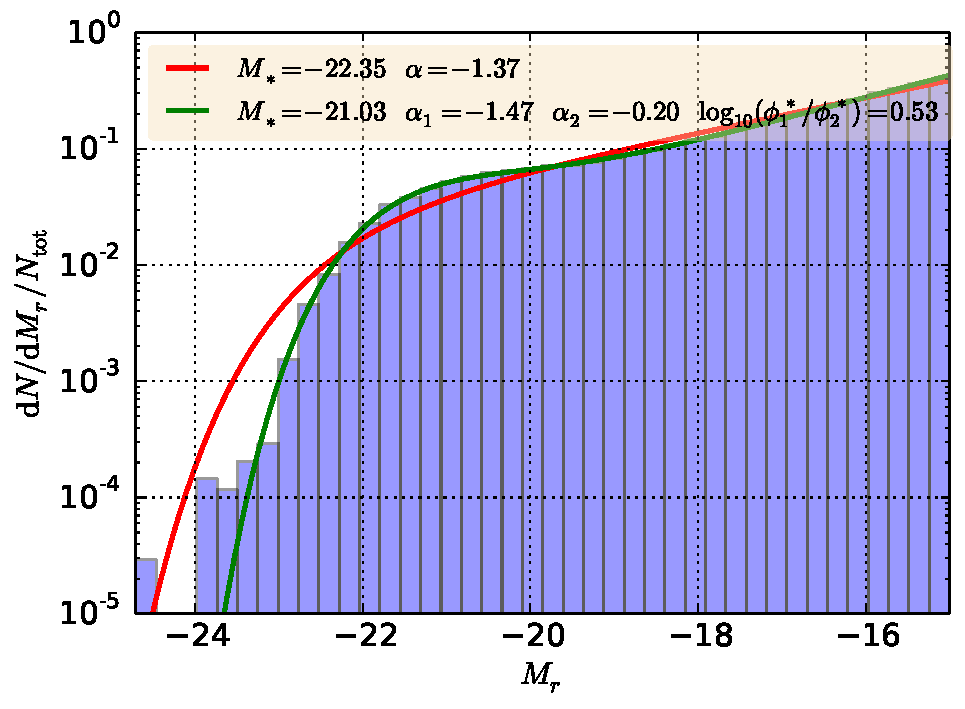
\includegraphics[width=0.7\linewidth]{figures/lf/guo_all}
    \caption{Fits of the galaxy luminosity distribution of the
        \textsc{Guo2010a} catalogue in the $r$ band. We fitted the simple
        Schechter function in green and the double Schechter function in red
        over the data in blue. Values in the legend correspond to the best fit
        parameters for each model, as described in the text.\label{fig:guo_all}}
\end{figure}
%
\com{Can't understand why the DS and SS give $M_*$ so different (two orders of
magnitude).}
%
The double Schechter fits better the data than the simple Schechter because
we can constrain the two populations of galaxies. We see that there is a low
population with high slope and a brighter population with a slope more
little. Differences with data for bright galaxies is due to the fact that
the number of galaxies with $M_r<-24$ is very low, in some bins there is
just one galaxy.
%
As expected, a Schechter and double Schechter functionals for the
luminosity function seem a good choice.

We want to see the modulation of the parameters with the halo mass. We take
galaxies in bins of the certain width in halo mass, and we compute the
parameters that fit well the data in each, as previously. This modulation is
represented in the figure (\ref{fig:modulation}).
%
\subsubsection{Flux limited sample}
%
With a flux-limited sample, we just need to rewrite the normalization to
take into account the total number of galaxies observed for a given redshift
$z$. We can proof it by rewriting the probability density in term of the
cumulative distribution. The probability that a galaxy have a magnitude
$\mathcal{M}$ superior to $M$ is given by:
%
\begin{equation}\label{eq:cumprobfluxlim}
    P\left(\mathcal{M}>M|z\right)=\cfrac{\int_{-\infty}^M{\phi\left({M'}\right){f\left({M'}\right)}\dd{M'}}}
    {\int_{-\infty}^{\infty}{\phi\left({M'}\right){f\left({M'}\right)}\dd{M'}}}
\end{equation}
%
where $f$ is the completeness function:
%
\begin{equation}
    f\left(M\right) = \begin{cases}
        1, &M^\mathrm{bright}\leq M \leq M^\mathrm{faint} \\
        0, & \mbox{else}
        \end{cases}
\end{equation}
%
Calculating the probability density is straightforward:
%
\begin{equation}
    P\left(\mathcal{M}>M|z\right)=\int_{-\infty}^M{p\left(M'|z\right)}\dd{M'}
\end{equation}
%
and so:
%
\begin{equation}
    p\left(M|z\right)=\ddp{P\left(\mathcal{M}>M|z\right)}{M}
\end{equation}
%
Finally:
%
\begin{equation}
    p\left(M_i|z_i\right)=\dfrac{\phi\left({M_i}\right)}{\int_{M_{\mathrm{bright}}\left({z_i}\right)}^{M_{\mathrm{faint}}\left({z_i}\right)}
    {\phi\left({M'}\right)\dd{M'}}}
\end{equation}
%
and this defines the new likelihood in the case of a flux limited sample.

We apply this to the incomplete sample generated with the mock algorithm we
have created (see Appendix~\ref{sec:mock}). The result of the application of
the MLE method on the mock catalog catalogue is shown on
Figure~\ref{fig:modulation}.
%
\begin{figure}
    \centering
    \begin{minipage}{\linewidth}
    \centering
    \subfloat[For a Schechter distribution]{%
        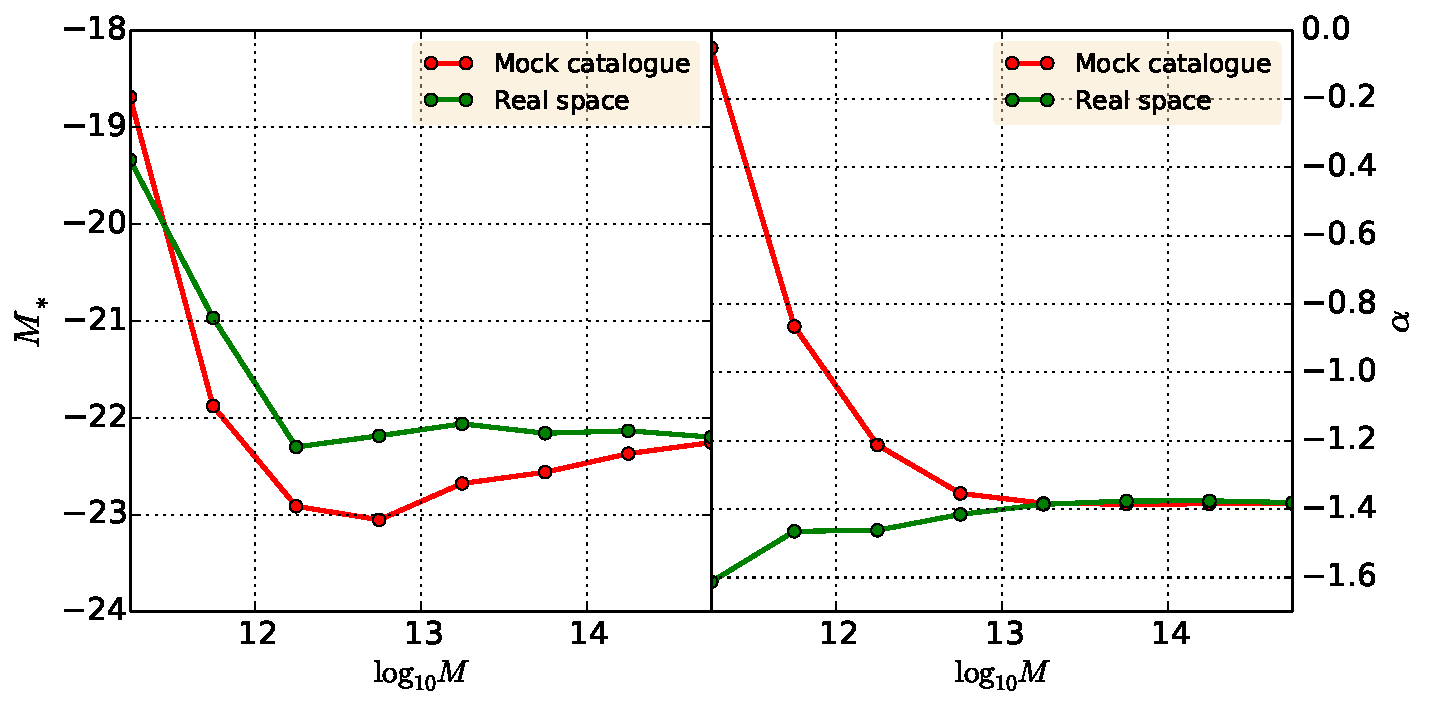
\includegraphics[width=0.85\linewidth]{figures/lf/schechter_fluxlimited_modulation}
    }
    \end{minipage}
    \begin{minipage}{\linewidth}
    \centering
    \subfloat[For a double Schechter distribution]{%
        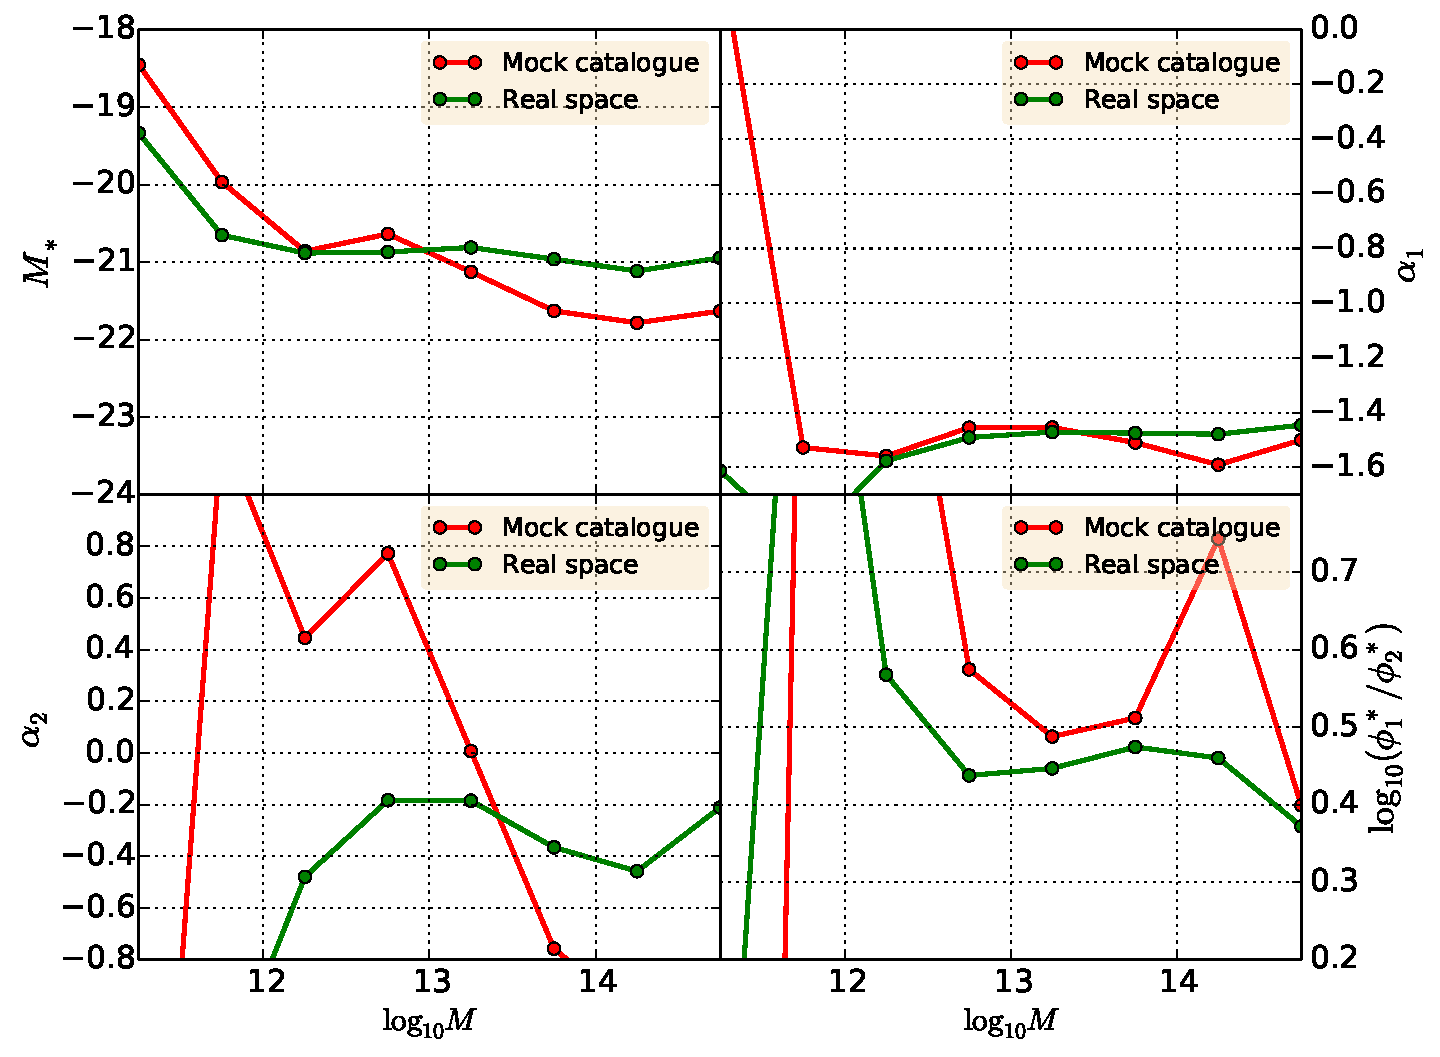
\includegraphics[width=0.85\linewidth]{figures/lf/double_schechter_fluxlimited_modulation}
    }
    \end{minipage}
    \caption{Modulation of the parameters of both Schechter and double
    Schechter luminosity distributions with the halo mass obtained from the
mock catalog (in red) and from the real space data (in
green).\label{fig:modulation}}
\end{figure}

The parameters are more or less recovered in flux-limited space. The bright
population isn't well recovered since its slope is very badly estimated and
the ratio between the two populations too. But, as the simple Schechter fit
shows it, the discrepancies with the real space appear for low mass halos.
Such groups are formed of faint galaxies disappearing at high redshift
because of the magnitude limit of observation. Thus, there is less galaxies
for statistics of low mass groups and the fit isn't good. Moreover, the
random filtering of boxes in the mock creation increases the cosmic variance
of the data for low mass groups. For the bright populations, the ratio
in number between the two  population is roughly of 5\%, and the statistics
are always poor for each bin of halo mass.
%
\begin{table}
    \centering
    \caption{Simple Schechter fit on the real space galaxy catalogue and on
    the redshift space mock catalogue.}
    \begin{tabular}{lcc}
        \toprule
        & $M_*$ & $\alpha$ \\
        \toprule
        Real space & -22.34 & -1.37 \\
        \midrule
        Redshift space & -22.40 & -1.31 \\
        \bottomrule
    \end{tabular}
\end{table}
%
\begin{table}
    \centering
    \caption{Double Schechter fit on the real space galaxy catalogue and on
    the redshift space mock catalogue.}
    \begin{tabular}{lcccc}
        \toprule
        & $M_*$ & $\alpha_1$ & $\alpha_2$ &
        $\log_{10}\left(\phi_2^*/\phi_1^*\right)$ \\
        \toprule
        Real space & -21.02 & -1.47 & -0.19 & 0.53 \\
        \midrule
        Redshift space & -21.09 & -1.43 & -0.05 & 0.57 \\
        \bottomrule
    \end{tabular}
\end{table}

To verify this assumption, and not incriminate a bad implementation of the
MLE for flux-limited samples, we applied the method on perfect samples of
galaxies. We generated an Universe with a given luminosity function and
applied the flux limit to galaxies in this region.
%
\newcommand{\mygamma}[2]{\Gamma\left(#1, \cfrac{#2}{L_*}\right)}
\remark{%
    Generating galaxies following a given luminosity function is done by the
    inverse transform sampling method. Let suppose that $F$ is a cumulative
    distribution function. This function is monotonic. Let $U$ be an random
    variable following a uniform distribution over $\left[0,1\right]$. If we
    define $Y=F^{-1}\left(U\right)$, this random variable follows the
    distribution of $F$. By definition, the cumulative distribution function
    of $Y$ is $p(Y \leq x) = p(F^{-1}\left(U\right) \leq x)$. Since the
    function is monotonic, $p(F^{-1}\left(U\right)\leq x)=p(U \leq
    F\left(x\right))$. The last expression is the cumulative distribution
    function for uniform distribution applied to the variable
    $F\left(x\right)$, which is directly equal to $F\left(x\right)$.

    The cumulative distribution function for the simple Schechter is:
    %
    \begin{equation}
        F\left(L\right)=\cfrac{\mygamma{\alpha+1}{L_{\min}} -
        \mygamma{\alpha+1}{L}}{\mygamma{\alpha+1}{L_{\min}} -
            \mygamma{\alpha+1}{L_{\max}}}
    \end{equation}
    %
    and for the double Schechter:
    %
    \begin{equation}
        F\left(L\right)=\cfrac{%
            \mygamma{\alpha_1+1}{L_{\min}} - \mygamma{\alpha_1+1}{L} +
            \cfrac{\phi_2^*}{\phi_1^*}\left(\mygamma{\alpha_2+1}{L_{\min}} -
            \mygamma{\alpha_2+1}{L}\right)
        }{%
            \mygamma{\alpha_1+1}{L_{\min}} - \mygamma{\alpha_1+1}{L_{\max}}+
            \cfrac{\phi_2^*}{\phi_1^*}\left(\mygamma{\alpha_2+1}{L_{\min}} -
            \mygamma{\alpha_2+1}{L_{\max}}\right)
        }
    \end{equation}

    Clearly, we can't inverse such cumulative distribution functions
    analytically. By interpolating them in the range of luminosities to
    generate, we can do an inversion and obtain the precious random
    variables following the Schechter distributions. This is fast and
    precise enough.

    The double Schechter can also be generated by two populations of simple
    Schechter functions. If $N_i$ is the number of galaxies
    following the distribution with parameters $\alpha_i$ and $\phi_i^*$,
    the ration between the two population is:
    %
    \begin{equation}
        \cfrac{N_2}{N_1} =
        \cfrac{\phi_2^*}{\phi_1^*}\times\cfrac{\mygamma{\alpha_2+1}{L_{\min}} -
        \mygamma{\alpha_2+1}{L_{\max}}}{\mygamma{\alpha_1+1}{L_{\min}} - \mygamma{\alpha_1+1}{L_{\max}}}
    \end{equation}
    %
    with $N_\mathrm{tot}=N_1+N_2$. But its easier to take the cumulative
    distribution function of the double Schechter, else we need to shuffle
    the resulting two populations from the simple Schechter generation.
}
%
We are enable to recover the simple Schechter parameters used to generate
the distribution in the flux limited sample. Using a double Schechter
distribution, parameters used for the generation are more difficult to
recover. Essentially for the bright population whose number is low
relatively to the faint one.

Results are also dependent of the initial guess chosen for the minimization.
This is a problem if we want to iteratively correct for missing galaxies in
MAGGIE, since we need it to be robust against this choice. Indeed, the group
population is varying along the iterative process and the modulation of
galaxy properties with halos will evolve, as our assumptions on the
luminosity function parameters.

Since it can be very difficult to correct our groups in a flux-limited
sample, we will just use doubly complete samples, where corrections are not
needed.
%
\section{Red and blue galaxies}
%
Galaxies form a bimodal distribution, mainly separated into red and blue
ones. From previous studies, their repartition inside galaxy groups isn't
the same. Using this segregation into MAGGIE should improve the group
selection and our measures of the environment.

This integration is done inside the probability of being in a group. We
compute a different probability if the galaxy is red or blue, by adjusting
the models according to the galaxy color. Such models are updated in the
iterative process, in order to get a relative independence of our results to
the adopted models.

Taking again the computation of the probability, if we know the fraction of
blue or red galaxies at a given radius to the group center, we can multiply
the density profile by this fraction, giving us the projected phase space
density of blue or red galaxies in halos. We have:
%
\begin{equation}
    g_\mathrm{halo}^i\left(R, v_z\right)=\int_R^{r_v} f_i\left(r\right) \rho\left(r\right)
    \cfrac{r}{\sqrt{r^2-R^2}} h\left(v_z|R,r\right) \dd{r}
\end{equation}
%
where $h\left(v_z|R,r\right)$ is the line of sight velocity distribution and
$f_i\left(r\right)$ is the fraction of $i$ galaxies, with
$i\in\left\{\mbox{red, blue}\right\}$. The fraction is model whose
parameters must be fitted to the data for each iteration with the set of
extracted groups. Since its a distribution function, this implies the use of
MLE with numerical computation of the integral, and a double integral for
the normalization of the density since:
%
\begin{equation}
    g_\mathrm{halo}^i\left(R, v_z\right) = \cfrac{\dd^2N}{\dd R\dd v_z}
\end{equation}

Supposing this computation can be easily done, there is still two problems.
\begin{itemize}
    \item The NFW profile is dependent of the concentration. Many studies
        shows that the concentration of blue and red galaxies inside halos
        is different. \note{Ask Gary for the articles.}.
    \item The probability needs to be normalized with the projected phase
        space density of interlopers. But we have no idea of their
        distribution when red and blue galaxies are separated. This needs to
        be extracted from mock catalogues, leading to densities not
        universal and dependent of the semi-analytical code used.
\end{itemize}
